
%-----------------------
%\input{wp-introduction}
%-----------------------

We summarize here a feasibility study~\cite{Mu2eII} of a
next-generation Mu2e experiment (Mu2e-II) that uses much of the
currently-planned facility and Project~X~\cite{ProjectX} beams to
achieve a sensitivity that is about a factor of ten beyond that of the
Mu2e experiment described in Section~\ref{cl:sec:mu2e}. A factor of
ten improvement will be interesting regardless of the outcome of Mu2e.
If the Mu2e experiment observes events completely consistent with
background expectations, then another factor of ten improvement in
sensitivity extends the reach to additional beyond-the-standard-model
parameter space.  If Mu2e observes a $3\sigma$ excess, then a Mu2e-II
upgrade would be able to definitively resolve the situation.  And if
Mu2e discovers charged-lepton-flavor-violating physics, then a Mu2e-II
upgrade could explore different stopping targets in an effort to
untangle the underlying physics.  By measuring the signal rate using
nuclear targets at various $Z$, Mu2e-II would have the unique ability
to resolve information about the underlying effective operators that
are responsible for the lepton-flavor-violating
signal~\cite{Kitano:2002mt,Cirigliano:2009bz}.



%-----------------------
%\input{wp-simulations}
%-----------------------
To estimate the signal acceptance and background prediction for
Mu2e-II scenarios we use \texttt{G4Beamline v2\_12}~\cite{g4bl}, which
is a simplified version of Geant4~\cite{GEANT4}.  Three sets of
simulated experiments are studied: the 8~\gev\ case which corresponds
to the Mu2e configuration, and potential Project~X upgrades
corresponding to protons with 1 or 3~\gev\ of kinetic energy.  In all
instances the full Mu2e solenoid system is simulated including all
collimators, the Production Solenoid heat and radiation shield, the
antiproton window, and the magnetic field.  The stopping target
geometry is described in~\cite{Mu2eCDR} and is left unchanged for the
different scenarios.
 

The timing distribution of the proton pulse in \texttt{G4Beamline} is
modeled as a delta function located at $t = 0$~ns.  In order to get a
more accurate estimate of the experimental sensitivity we convolute
the relevant timing distributions with the expected shape of the
proton pulse as estimated using dedicated simulations of the Mu2e
proton beam.  For Project~X, the width of the proton pulses are
expected to be $\pm 50$~ns for 100 kW of beam power~\cite{bobT}, which is
about a factor of two narrower than what will be used for Mu2e.  So,
for the Project~X studies we assume the same proton pulse shape as
supplied for Mu2e, but reduce the width of the pulse by a factor of
two.  Most pions decay before reaching the stopping target, and due to
this short lifetime it isn't practical to study the pion backgrounds
if the decay is simulated.  Instead, in these studies all charged
pions pions are propagated through to the stopping target and events
are weighted by the survival probability.
 

The stopping-time distributions for muons and pions are studied in
Ref.~\cite{Mu2eII} and are used for the estimations of background and
signal acceptance below.  We find that the stopping-time distributions
are largely independent of the stopping target material.
   

\begin{table}[tb]
  \centering
  \begin{tabular}{rccc} \hline\hline
           & lifetime (ns) & capture fraction & decay fraction \\ \hline
  Aluminum & 864           & 0.61            & 0.39 \\
  Titanium & 297           & 0.85            & 0.15 \\ \hline\hline
  Gold     &  72           & 0.97            & 0.03     \\ \hline\hline
  \end{tabular}
  \caption{The lifetime of the bound muon and the muon capture and decay     
    fractions for various stopping target nuclei that affect the 
    sensitivity estimates for Mu2e-II. 
  }
  \label{cl:tab:nucleistuff}
\end{table}
  
Relevant timing distributions for the Mu2e experiment are shown in the
top panel of Fig.~\ref{cl:fig:timing} for an aluminum stopping
target. Since the $\pi^-$-N interaction is strong, the pion
capture-time distribution is assumed to be the same as the pion
arrival-time distribution.  For muons, the capture/decay rate is
characterized by a falling exponential.  The fractions of bound muons
that are captured or that decay-in-orbit (DIO) are also nuclei
dependent.  These nuclei-dependent characteristics affect the
sensitivity of a given experiment and are listed in
Table~\ref{cl:tab:nucleistuff} for the stopping-target nuclei we
considered~\cite{Suzuki:1987jf}.  The muon decay-time distribution is
shown in the top panel of Fig.~\ref{cl:fig:timing} as the blue dashed
line.  In this figure the timing distributions are folded over modulo
1695~ns in order to account for contributions from previous proton
pulses.

The bottom panel of Fig.~\ref{cl:fig:timing} shows the Project~X
3~\gev\ scenario, where the proton pulse width is half that of the
8~\gev\ configuration, and both aluminum, titanium, and gold are
considered as a stopping target~\footnote{Note that the arrival times
for stopped particles are slightly earlier for titanium than for
aluminum although it isn't depicted in the figure.}. Because the proton
pulse width is narrower, the live gate can be increased in the
Project~X scenario~\cite{MoveLiveGate}.  The same exercise was
performed for the Project~X 1~\gev\ scenario and with the exception of
the stopping rates, the parameters of the timing distributions for the
1~\gev\ case are very similar to those of the 3~\gev\ case.  The
relavant quantities associated with Fig.~\ref{cl:fig:timing} are
included in Ref.~\cite{Mu2eII} and used below to predict the
background and signal rates for each scenario.


% in Table~\ref{cl:tab:stopping}.
%\begin{table}[tb] 
%  \centering
%  \begin{tabular}{lccccc}\hline\hline
%\multicolumn{6}{l}{Mu2e at 8~\gev (live gate $670 < t < 1595$ ns)}  \\  
%                     & \multicolumn{2}{c}{Aluminum target} &\hspace*{0.15in}  && \\
%                                         & Muons         & Pions         &&&\\  \hline
%    Stops/POT                             & \sn{1.61}{-3} & \sn{6.82}{-7} &&&\\
%    Stop Time (Mean)                      & 259.8 ns      & 192.1 ns      &&&\\
%    Stop Time (rms)                       & 86.58 ns      & 47.6 ns       &&&\\
%    Fraction of $\mu$-decays in live gate & 0.489         & ---           &&&\\
%    Fraction of $\pi$-decays in live gate &  ---          & \sn{3.93}{-11}&&&\\
%\hline
%\hline
%\multicolumn{6}{c}{} \\
%\multicolumn{6}{l}{Mu2e-II at 1~\gev(live gate $670 < t < 1645$ ns)}  \\
%                     & \multicolumn{2}{c}{Aluminum target} &\hspace*{0.15in} & \multicolumn{2}{c}{Titanium target} \\
%                     & Muons         & Pions                      & & Muons         & Pions               \\  \hline
%    Stops/POT        & \sn{1.44}{-4} & \sn{6.44}{-8}              & & \sn{1.87}{-4} & \sn{1.40}{-7}       \\
%    Stop Time (Mean) & 257.4 ns      & 189.7 ns                   & & 242.3 ns      & 176.7 ns            \\
%    Stop Time (rms)  & 78.46 ns      & 34.3 ns                    & & 76.83 ns      & 33.5 ns             \\
%    Fraction of $\mu$-decays in live gate & 0.496 & ---           & & 0.266         & ---                 \\
%    Fraction of $\pi$-decays in live gate &  ---  & \sn{1.40}{-11} & &  ---          & \sn{4.51}{-12}      \\
%\hline
%\hline
%\multicolumn{6}{c}{} \\
%\multicolumn{6}{l}{Mu2e-II at 3~\gev (live gate $670 < t < 1645$ ns)}  \\
%                     & \multicolumn{2}{c}{Aluminum target} &\hspace*{0.15in} & \multicolumn{2}{c}{Titanium target} \\
%                    & Muons              & Pions                 & & Muons         & Pions               \\  \hline
%    Stops/POT        & \sn{6.69}{-4}      & \sn{2.90}{-7}         & & \sn{8.68}{-4} & \sn{6.35}{-7}       \\
%    Stop Time (Mean) & 257.8 ns           & 190.1 ns              & & 242.6 ns      & 177.1 ns            \\
%    Stop Time (rms)  & 79.03 ns           & 34.5 ns               & & 77.34 ns      & 33.7 ns             \\
%    Fraction of $\mu$-decays in live gate & 0.497 & ---           & & 0.269         & ---                 \\
%    Fraction of $\pi$-decays in live gate &  ---  & \sn{1.14}{-11} & &  ---          & \sn{4.74}{-12}      \\
%    \hline\hline
%  \end{tabular}
%  \caption{Stopped muon and pion quantities for a Mu2e and for the Mu2e-II Project~X scenarios
%  with a narrower pulse width and 1.   The fraction of decays/captures
%  includes contributions from the previous proton bunch.}
%  \label{cl:tab:stopping}
%\end{table}



\begin{figure}[htb]
  \centering
  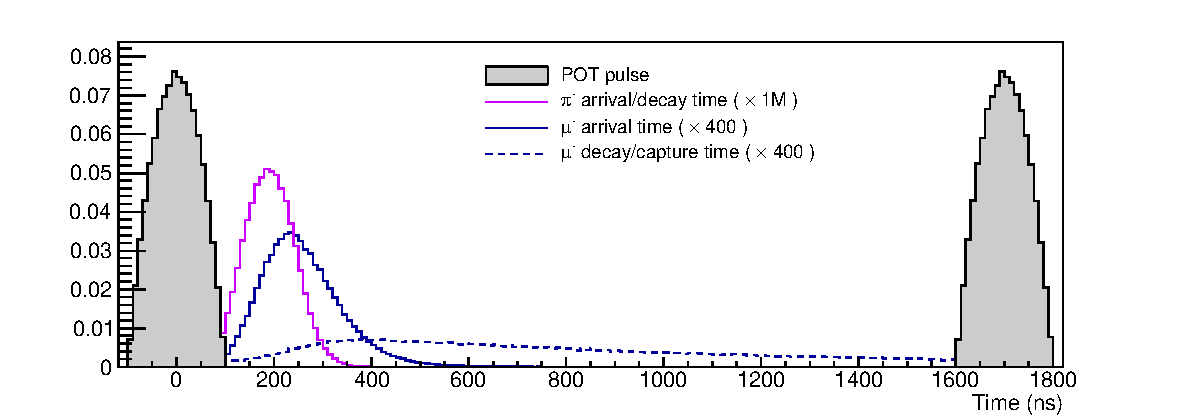
\includegraphics[width=0.75\textwidth]{ChargedLeptons/Figures/muon_fullCycle_Al_8GeV_Alt.pdf}
  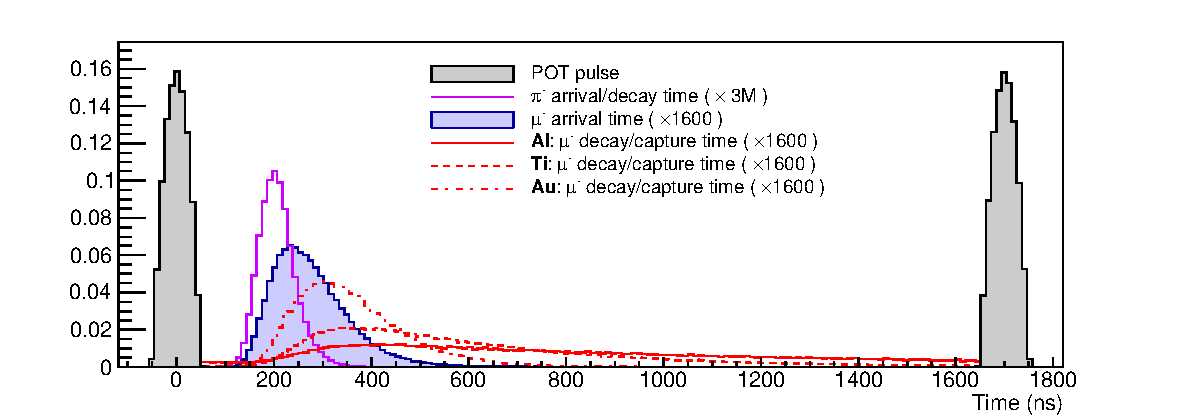
\includegraphics[width=0.75\textwidth]{ChargedLeptons/Figures/muon_fullCycle_AlTiAu_3GeV_Alt.pdf}
  \caption{Timing distribution for the 8-GeV Mu2e case (top) and the 3-GeV Project~X case (bottom).  Shown
  here is a figurative POT pulse width, the arrival time of the
  charged pions and muons, and the decay-time distribution of the
  muons on aluminum, titanium, and gold.}
  \label{cl:fig:timing}
\end{figure}


We also produced the muon decay-time distribution for a gold stopping
target as shown in Fig.~\ref{cl:fig:timing}.  Since the lifetime of
the bound muon is so small (72~ns) the fraction of muon
decays/captures that occur within the live gate is quite small -- only
1.22\% for a live gate of $670 < t < 1645$~ns.  Since the muon
decay-time distribution has such a large overlap with the pion arrival
time distribution, it's clear that it will be difficult to achieve a
reasonable signal acceptance while sufficiently suppressing the RPC
background.  To achieve the necessary pion/muon separation requires a
dedicated study of alternative transport systems and is beyond the
scope of this study. We do not further consider the gold stopping
target.



%\input{wp-backgrounds}

We estimate the backgrounds for several Mu2e-II scenarios as described in Ref.~\cite{Mu2eII}.  These estimates assume that the detector performance for Mu2e-II is unchanged relative to the currently planned Mu2e detector.  Simulation studies of detector performance at the higher Mu2e-II intensities indicate that this can be achieved with modest upgrades as discussed below.

%We use the quantities from Ref.~\cite{Mu2eII} to estimate the
%backgrounds for several Mu2e-II scenarios.  No additional simulation
%work was done aside from the simulations described above.
%Consequently, we here estimate the Mu2e-II backgrounds by scaling from
%the Mu2e backgrounds which were derived using full simulation as
%described in~\cite{Mu2eCDR} and references therein.  In numbers quoted
%in Ref.~\cite{Mu2eII} the stopping rates are larger for titanium than
%for aluminum due to the fact that in the simulations we left the
%stopping-target geometry unchanged and that titanium is heavier and at
%a larger $Z$.  In that configuration a titanium stopping target would
%also have a poorer momentum resolution.  In the estimates below, we
%assume that reducing the titanium stopping-target mass so that it gave
%the same stopping rates as aluminum would yield the same momentum
%resolution. Thus, in these estimates, we always use the aluminum
%stopping yields for a given proton beam energy and scale from the Mu2e
%background estimates assuming that the same detector performance for
%Mu2e-II.


For each beam scenario target nuclei we estimate the number of protons
on target ($N_{\mathrm{POT}}$) required to improve the signal
expectation by a factor of ten. This is done by scaling from the Mu2e
experiment by the number of stopped muons per POT, the muon capture
fraction, and the fraction of muon capture/decay that occur in the
signal timing window.  We then take the resulting number of POT and
calculate the required beam power, and the number of muon and pion
stops per kW, assuming the same run time for Mu2e-II as Mu2e, namely a
three-year run with $\sn{2}{7}$ seconds of run time per year with
proton pulse spacing of 1695~ns.  These studies predict that between
\sn{8.7}{21} and \sn{5.3}{22} $N_{\mathrm{POT}}$ are required
depending on the beam and target scenario which corresponds to 70--150
kW of beam power.  The detailed results of these calculations are
given in Ref.~\cite{Mu2eII}.


%The results of these calculations are given in Table~\ref{cl:tab:npot}.
%\begin{table}[tb]
%  \centering
%  \begin{tabular}{llcccc} \hline\hline
%  & &\hspace*{0.15in} & 3~\gev\ &\hspace*{0.15in} & 1~\gev\ \\ \hline
%  \multirow{4}{*}{Aluminum (3y run)\hspace*{0.10in}} 
%    & $N_{\mathrm{POT}}$ & & \sn{8.7}{21} & & \sn{4.0}{22} \\
%    & beam power (kW)    & & 72           & & 112 \\
%    & $\mu$ stops / kW   & & \sn{8.0}{16} & & \sn{5.2}{16} \\   
%    & $\pi$ stops / kW   & & \sn{3.5}{13} & & \sn{2.3}{13} \\ \hline
%  \multirow{4}{*}{Titanium (3y run)\hspace*{0.10in}} 
%    & $N_{\mathrm{POT}}$ & & \sn{1.1}{22} & & \sn{5.3}{22} \\
%    & beam power (kW)    & & 94           & & 147 \\
%    & $\mu$ stops / kW   & & \sn{8.0}{16} & & \sn{5.2}{16} \\   
%    & $\pi$ stops / kW   & & \sn{3.5}{13} & & \sn{2.3}{13} \\ \hline\hline
%  \end{tabular}
%  \caption{Calculated number of POT necessary for Mu2e-II to achieve a 
%    $\times 10$ smaller single-event-sensitivity than Mu2e and the
%    corresponding beam power and muon and pion stopping rates.  The beam
%    power is calculated assuming the same run time (three-year run with 
%    $\sn{2}{7}$ s/year) and proton pulse spacing (1695 ns) as Mu2e.
%  }
%  \label{cl:tab:npot}
%\end{table}


Several background sources will be reduced or remain minimal at
Mu2e-II due to the improved beam characteristics compared to Mu2e.
For example, there are no antiproton-induced backgrounds for the
Project~X scenarios since both 1~\gev\ and 3~\gev\ kinetic energy
protons are below the proton-antiproton production threshold.  The
radiative pion capture background is kept under control for Mu2e-II
owing to the narrower proton pulse widths at Project~X and owing to
the significantly improved extinction provided by Project~X beams.
Late-arriving backgrounds, such as $\pi$ decay-in-flight, are also
kept under control by the decrease in the extinction ratio relative to
those same quantities for Mu2e.
   
The cosmic ray background is independent of $N_{\mathrm{POT}}$ and
beam power and depends only on the live time of the experiment. Since
we assume that Mu2e-II will have the same run time (three-year run
with $\sn{2}{7}$ s/year) and proton pulse spacing (1695~ns) as Mu2e,
the only difference is in the duty factor (which increases from 30\%
to 90\%) and the live-gate fraction. We scale the current Mu2e
estimate for the cosmic-ray-induced backgrounds to account for these
differences.  We assume that the veto efficiency for Mu2e-II is
unchanged relative to Mu2e (99.99\% ). For a Project~X (PX) driven
Mu2e-II experiment, the resulting cosmic-ray-induced background is
$0.16$ events.

Some backgrounds scale linearly with the number of stopped muons, such
as radiative muon captures and muon decay in orbit, and these can't be
mitigated through improved beam characteristics.  Radiative muon
capture is a negligible background for Mu2e and remains so for
Mu2e-II.

The $\mu$ decay-in-orbit background is calculated assuming that the
probability that a DIO event survives the reconstruction and selection
requirements for Mu2e-II are unchanged relative to Mu2e,
$\alpha_{\mathrm{DIO}} = \sn{1.9}{-18}$~\cite{Mu2eCDR}.  Note that
this implicitly assumes that the momentum resolution, and in
particular the magnitude and shape of the high-side tail, is unchanged
relative to Mu2e. In addition, it assumes that the shape of the DIO
spectrum for a titanium stopping target is the same as the shape of
the spectrum for aluminum stopping target.  A Mu2e-II experiment with
an aluminum stopping target and a $\times 10$ better sensitivity than
Mu2e is therefore expected to have a DIO background $\times 10$ larger
than Mu2e.  The only mitigations are to make more stringent momentum
requirements or to redesign the tracker and the upstream material
(e.g. stopping target, internal proton and neutron absorbers, etc.) to
improve the momentum resolution.  Studies of the DIO background
performed for the Mu2e experiment show that it is unlikely that for an
aluminum stopping target, more stringent selection requirements alone
could mitigate a ten-fold increase in the DIO background without a
significant reduction in signal sensitivity.  For the increased
sensitivity of a Mu2e-II experiment an improved momentum-scale
calibration may also be required to reduce the DIO background.  This
would not necessarily be the case for a Mu2e-II experiment that uses a
titanium stopping target~\cite{DIOComment}.

The summary of the background estimates for Mu2e-II are given in
Table~\ref{cl:tab:PXBgd} along with the estimate for Mu2e.

\begin{table}[t]
  \centering
  \begin{tabular}{llcrcrcr} \hline\hline
    & & \hspace*{0.15in} & \multicolumn{1}{c}{Mu2e} &\hspace{0.15in} &\multicolumn{3}{c}{Mu2e-II} \\
    & & & \multicolumn{1}{c}{8~\gev } & &\multicolumn{3}{c}{1 or 3~\gev } \\
    & & & \multicolumn{1}{c}{Al.} & & \multicolumn{1}{c}{Al.}  &\hspace*{0.1in} & \multicolumn{1}{c}{Ti.} \\ \hline
    Category      & Source                     
    & &\multicolumn{5}{c}{Events} \\ \hline
    \multirow{2}{*}{Intrinsic} 
                  & $\mu$ decay in orbit       
    & & 0.22 & & 2.14 & & $0.58^*$  \\ 
                  & radiative $\mu$ capture    
    & & $<0.01$ & & $<0.01$ & & $<0.01$  \\ \hline
    \multirow{4}{*}{Late Arriving}
                  & radiative $\pi$ capture    
    & & 0.03 & & 0.04 & & 0.05  \\
                  & beam electrons             
    & & $<0.01$ & & $<0.01$ & & $<0.01$  \\
                  & $\mu$ decay in flight      
    & & 0.01 & & $<0.01$ & & $<0.01$   \\
                  & $\pi$ decay in flight      
    & & $<0.01$ & & $<0.01$ & & $<0.01$  \\ \hline
    \multirow{3}{*}{Miscellaneous}
                  & antiproton induced        
    & & 0.10 & & -- & & --  \\
                  & cosmic-ray induced         
    & & 0.05 & & 0.16 & & 0.16   \\
                  & pat. recognition errors    
    & & $<0.01$ & & $<0.01$ & & $<0.01$  \\ \hline
    Total Background &                         
    & & 0.41 & & 2.34 & & 0.79  \\ \hline\hline
  \end{tabular}
  \caption{A summary of the current Mu2e background estimates and 
    estimates of how the backgrounds would scale for a next generation
    Mu2e experiment, Mu2e-II, that employs Project~X beams at 1 or 
    3~\gev\ and an aluminum or titanium stopping target. For a given 
    stopping target, the difference in background yields between a 
    1~\gev\ or a 3~\gev\ proton beam is about 10\%.  The total 
    uncertainty on the total Mu2e background is estimated to be 
    about 20\%. We've added a $*$ to the DIO estimate for the titanium
    stopping target to emphasize the fact that this number is expected
    to change once more detailed 
    studies have been completed~\cite{DIOComment}.
  }
  \label{cl:tab:PXBgd}
\end{table}


%\input{wp-upgrades}

Several components of the Mu2e experiment may need to be upgraded to
handle the higher rates and physics requirements of Mu2e-II.  To
accommodate beam power in the 80kW-110kW range estimated for Mu2e-II
several aspects of the Target and Target Hall would have to be
upgraded.  The proton beam dump would need improved cooling and the
production target would need to be redesigned.  A new production
target design would likely require modifications to the remote target
handling system.  Depending on the proton beam energy and the PS
configuration, it may be necessary to redesign some portions of the
Mu2e beam line just upstream of the PS. Since the extinction in the
Project~X scenarios is a factor 100 smaller than for Mu2e, the
Extinction Monitor system would have to be upgraded to increased
acceptance/sensitivity.  It is expected that even at the increased
rates and beam power discussed earlier, the transport solenoid and
detector solenoid should be able to operate reliably for a Mu2e-II
run. For the production solenoid, the limiting factors are the peak
power and radiation damage it would incur at the increased beam power.
For example, the Production Solenoid heat and radiation shield , which
is currently planned to be fabricated from bronze, could sustain
higher peak power if replaced with tungsten~\cite{Mu2eII}.

Although the beam power increases by a factor of 10 or more, the
instantaneous rates only increase by a factor of 3-5 owing to the
increased duty factor expected from Project~X.  This has important
consequences for the viability of reusing much of the currently
planned Mu2e detector apparatus for a next generation Mu2e-II.  For
example, the current Mu2e tracker is being designed to handle
instantaneous rates higher than what is currently estimated.
Simulation studies in which the instantaneous rates are increased by
factors of two or four have been performed.  These studies indicate
that at four times the nominal rates the tracker reconstruction
efficiency only falls by about 5\% while maintaining the same momentum
resolution.  Thus, these studies indicate that the Mu2e tracker would
be able to handle the Project~X rates.  Simulation studies are
necessary to quantify the degree to which the increased rates affect
the calorimeter's performance.  If it turns out that the expected
performance is not sufficient to meet the Mu2e-II physics
requirements, then it may be necessary to upgrade to faster readout
electronics or to a faster crystal ({\it e.g.} BaF$_2$).  Regardless of the
outcome of the simulation studies, the photo sensors will likely
require replacement owing to radiation damage incurred during Mu2e
running.  The performance of the LYSO crystals is not expected to be
significantly affected by the radiation dose incurred during Mu2e
running.

The current design of the cosmic ray veto system should be adaptable
to the case with a factor of 3--5 increase in rate with only minor
upgrades required and these may only be needed in the most intense
radiation regions of the veto system.  Experience from the first run
of the Mu2e experiment will be crucial in quantifying limitations of
the system for future intensity upgrades.  Improved shielding will
likely be required in the highest radiation regions to reduce
incidental rates in the veto counters.



%\input{wp-conclusion}


We investigated the feasibility of a next generation Mu2e experiment
(Mu2e-II) that uses as much of the currently planned facility as
possible and Project~X beams to achieve a sensitivity that's about a
factor of ten better than Mu2e.  Based on these studies we conclude
that a Mu2e-II experiment that reuses a large fraction of the
currently planned Mu2e apparatus and provides a $\times 10$ improved
sensitivity is feasible at Project~X with 100-150 kW of 1 or 3~\gev\
proton beams.  Aside from the DIO background, which requires improved
momentum resolution to mitigate, the remaining backgrounds are kept
under control due to important features of Project~X.  The narrower
proton pulse width and expected excellent intrinsic extinction are
both important to mitigating the RPC background.  The excellent
intrinsic extinction is also important in mitigating backgrounds from
late arriving protons such as $\mu$ and $\pi$ decay-in-flight and beam
election backgrounds.  A beam energy below the proton-antiproton production
threshold eliminates the antiproton induced backgrounds.  The high
duty factor expected for Project~X is important since it enables a
ten-fold improvement in sensitivity over a reasonable timescale while
necessitating only a modest increase (a factor of 3-5, depending on
scenario) in instantaneous rates at the detectors.  Because the
instantaneous rates increase only modestly, we believe that Mu2e-II
could reuse the currently planned Mu2e apparatus with only modest
upgrades necessary.
